\section{Observations}

\emph{TauRoast} was provided to us in the form of an
email which described, in prose, how to obtain the source,
build the program, and run it correctly on one specific
machine at our home institution, with no particular guarantee that
it will run anywhere else in the world.
Although this starting point may seem extreme, it is
perfectly natural for collaborators to share configurations
with each other in this form, and to rely on the presence
of a working environment with appropriate dependencies already
installed.  From this starting point, the authors played the
role of curators, whose job it is to prepare the application
for permanent archival.

First, we elaborated the email instructions into an
executable script that obtains the dependencies and then
executes the analysis.  The script declares the necessary
environment variables, downloads and checks out the necessary source code,
builds it appropriately, calls initialization scripts in
the dependent software, and then runs the analysis.
A few rounds of correction with the original author were necessary
to obtain all the dependencies and run the artifact correctly.
(The original instructions introduced in the email also indicated how to run the application
within a production batch system.  For the purposes of preservation,
we consider the execution infrastructure to be distinct from the application,
and leave it out of consideration for now.)

The process of elaborating the program into a script revealed
several observations about this type of application:

\begin{itemize}

\item {\bf Many Explicit External Dependencies.}  TauRoast depends on a large number of
external dependencies, each with a different access method and data source.
While we knew in advance that it depended upon the large CMSSW distribution,
it was not apparent until elaborating the script that it depended upon
two different Github repositories for the Tau source,
a CVS server at CERN for some configuration information, a public web page
for the PyYAML library, and the public home page of a Notre Dame student
for one missing header file.  (The latter is particularly troubling!)
While, at some level, the authors and users of these software know of these dependencies, they are often missing in
informal communications or forgotten once the dependency is installed.
However, once known, they are at least expressed explicitly within the script.

\item {\bf Many Implicit Local Dependencies.} A much harder problem is that the
application assumed the presence of many different components in the local
filesystem view. It would be tempting to capture all of these by simply
storing a virtual machine image containing the local filesystem. However,
the application depended on no less than {\bf five} networked filesystems
available on a particular machine available to the author:
the data to be analyzed was stored on an HDFS~\cite{borthakur2008hdfs} cluster,
some configuration data was stored on a CVMFS~\cite{blomer2011cernvm} filesystem,
and a variety of software tools were on an NFS~\cite{howard1988scale},
PanFS~\cite{welch2008scalable} and AFS~\cite{sandberg1985design} systems.
The original authors were not aware of many of these dependencies,
because they simply relied on local administrators to configure the
software and make it available.

\item {\bf Configuration Complexity.}  As a means of controlling the complexity
of dependent software packages, the high energy physics community has developed
a number of tools that perform run-time configuration and consistency checks
of the available software.  {\tt scram} is the software management tool used
by the CMS experiment.  Before running any code, {\tt scram} is used to locate
the appropriate version of software,  set environment variables such as the PATH, run any
tool-specific configuration, and do the same for all software on which it depends.
If the correct versions are not available, {\tt scram} halts and emits an error.
While this procedure has great value for consistency, it also introduces a significant cost
because it involves a large number of nested scripts traversing a filesystem,
repeatedly looking up metadata.  In our example, the time to perform this configuration
with a cold cache is about 14 minutes, which is almost as large as the actual analysis
run, which takes 20 minutes.

\begin{figure*}[t]
\centering
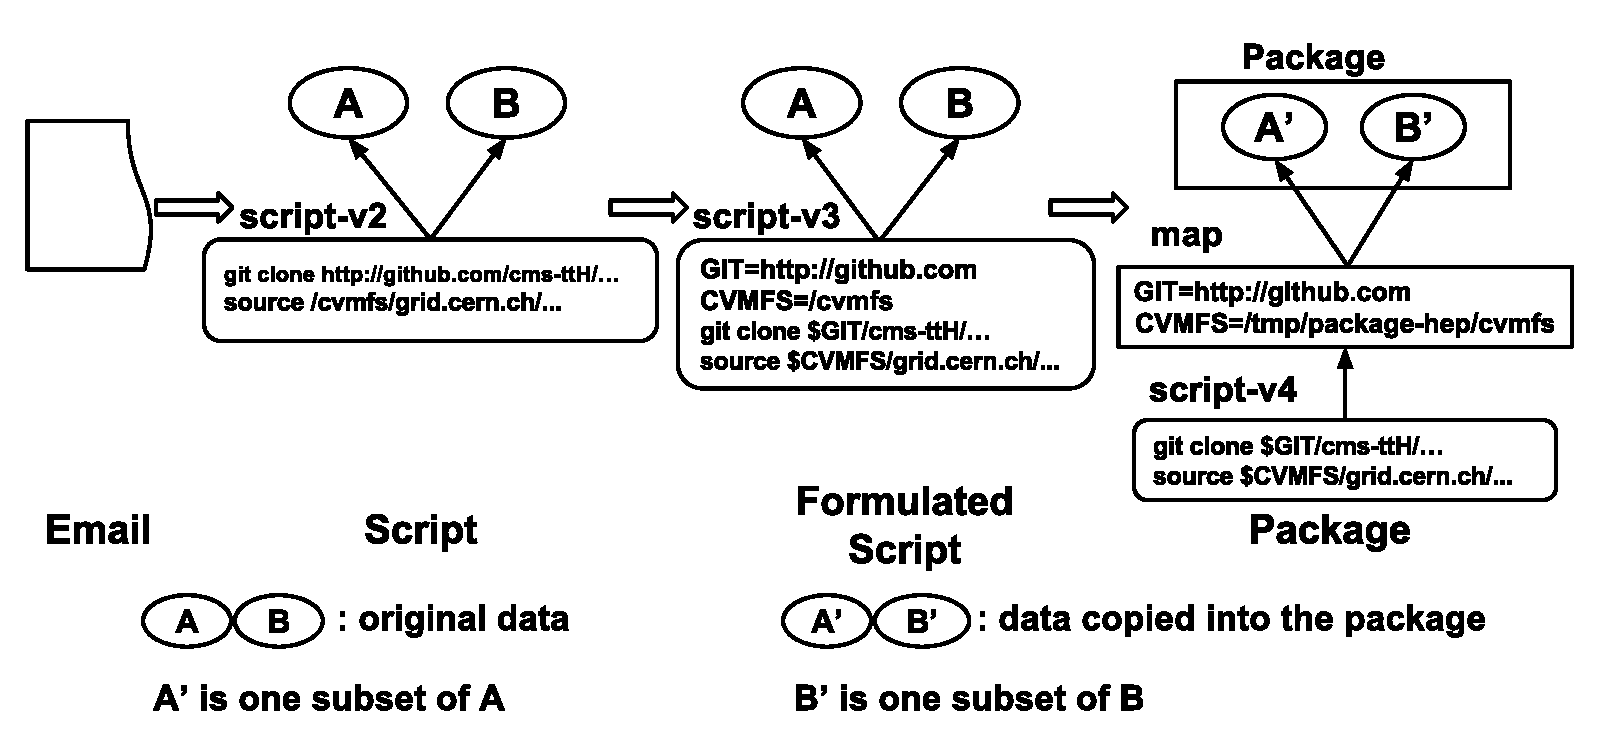
\includegraphics[width=.8\textwidth]{version-evolution.eps}
\caption{Version Evolution}
\label{fig:version-evolution}
\end{figure*}

\item {\bf High Selectivity.}  Although the total size of the resources accessed by this
program is very large, the size of the data and software actually used are much smaller.
Often, an entire repository or data source is named within the script, but the program
only needs a handful of items from that source.  For example, the data is stored on an
HDFS filesystem with 11.6TB of data, but only 20GB are actually consumed by the program. 
The reason for this great reduction is at first each BEAN event contains a large amount of information, and the TauAnalysis throws away a lot of the irrelevant event information, keeping only the relevant bits.
The CMSSW repository is 88.1GB in total
but only 448.3MB of source is checked out, and the actually used software only
measured 6.3MB.  In a few cases, a source of software is named but never actually accessed.
(For example, our original script includes the Open Science Grid software stack in the PATH, but does not actually use it.)
We suspect that end users are accustomed to missing dependencies and thus get in the habit of adding commonly used software,
whether it is needed or not.

\item {\bf Rapid Changes in Dependencies.}  Over the course of three months
between collecting the initial email, analyzing the program, and writing this
paper, the computing environment continuously changed.  The CMSSW software
distribution released a new version, the target execution environment was upgraded
to a new operating system, and the application deprecated the use of CVS for obtaining
the software.  While the users of this software seem be accustomed to constant change,
any preservation technique will have to be very cautious about relying upon an
external service, even one that may appear to be highly stable.

\end{itemize}

\if 0

\begin{table}
    \centering
    \begin{tabular}{|l|}
        \hline
        {\bf Version 1: Email}\\ \hline
        1. Create a CMS release,\\
            \hspace{9pt} e.g. {\tt cmsrel CMSSW\_5\_3\_11\_patch3} \\
        2. Install the BEAN packages as the instructions: \\
            \hspace{9pt} {\tt \url{https://github.com/cms-ttH/BEAN/blob/...}}\\
        3. Install grid-control: \\ 
            \hspace{9pt} {\tt svn co \url{https://ekptrac.physik.uni-ka/...}} \\
        4. INstall the TauAnalysis package: \\
           \hspace{9pt} {\tt git clone \url{https://github.com/matz-e/...}} \\
           \hspace{9pt} {\tt scram b -j32} \\
        5. Fix grid\_control.cfg and run it. \\
        6. Perform the actual tau roast program. \\ 
        \hline
        {\bf Version 2: Script}\\ \hline
        {\tt setenv CMSSW\_BASE CMSSW\_5\_3\_11\_patch3} \\
        {\tt cmsrel \$HOME/\$CMSSW\_BASE} \\
        {\tt cvs co -r V03-09-23 PhysicsTools/PatUtils} \\
        {\tt git clone \url{https://github.com/cms-ttH/BEAN.git}} \\
        {\tt wget -r \url{http://nd.edu/~abrinke1/...}} \\
        {\tt scram b -j32} \\
        {\tt wget \url{http://pyyaml.org/download/pyyaml/PyYAML...}}\\
        \#the experiment data is from HDFS \\
        {\tt cd \$HOME/\$CMSSW\_BASE/src/PyYAML-3.10}\\
        {\tt cmsenv}\\
        {\tt python setup.py install --user} \\
        {\tt scripts/roaster data/generic\_ttl.yaml} \\ 
        \hline
        {\bf version 3: Formulated Script} \\ \hline
        {\tt setenv CMSSW\_BASE CMSSW\_5\_3\_11\_patch3} \\
        {\tt setenv {\bf GIT} \url{https://github.com}} \\
        {\tt setenv {\bf PYYAML} \url{http://pyyaml.org}} \\
        {\tt setenv {\bf ND} \url{http://nd.edu}} \\
        {\tt cmsrel \$HOME/\$CMSSW\_BASE} \\
        {\tt cvs co -r V03-09-23 PhysicsTools/PatUtils} \\
        {\tt git clone \${\bf GIT}/cms-ttH/BEAN.git} \\
        {\tt wget -r \${\bf ND}\url{/~abrinke1/ElectronEffectiveArea.h}} \\
        {\tt scram b -j32} \\
        {\tt wget \${\bf PYYAML}/download/pyyaml/PyYAML...}\\
        \#the experiment data is from HDFS \\
        {\tt cd \$HOME/\$CMSSW\_BASE/src/PyYAML-3.10}\\
        {\tt cmsenv}\\
        {\tt python setup.py install --user} \\
        {\tt scripts/roaster data/generic\_ttl.yaml} \\ 
        \hline
       {\bf Version 4: Fine-Grained Toolkit - Package}\\ \hline
        {\tt setenv CMSSW\_BASE CMSSW\_5\_3\_11\_patch3} \\
        {\tt setenv {\bf GIT} \url{https://github.com}} \\
        {\tt setenv {\bf PYYAML} \url{http://pyyaml.org}} \\
        {\tt setenv {\bf ND} \url{http://nd.edu}} \\
        {\tt cmsrel \$HOME/\$CMSSW\_BASE} \\
        {\tt cvs co -r V03-09-23 PhysicsTools/PatUtils} \\
        {\tt git clone \${\bf GIT}/cms-ttH/BEAN.git} \\
        {\tt wget -r \${\bf ND}\url{/~abrinke1/ElectronEffectiveArea.h}} \\
        {\tt scram b -j32} \\
        {\tt wget \${\bf PYYAML}/download/pyyaml/PyYAML...}\\
        \#the experiment data is from HDFS \\
        {\tt cd \$HOME/\$CMSSW\_BASE/src/PyYAML-3.10}\\
        {\tt cmsenv}\\
        {\tt python setup.py install --user} \\
        {\tt scripts/roaster data/generic\_ttl.yaml} \\ 
        \hline
    \end{tabular}
    \caption{Scripts of each Solution}
    \label{table:scripts}
\end{table}

\fi

